\subsection*{Problema 05}

\textbf{Enunciado:}
Calcular la integral indefinida:
\begin{align*}
I = \int \dfrac{dx}{1 - \cos x}
\end{align*}

\textbf{Solución:}
Para resolver la integral dada, utilizaremos una identidad trigonométrica del ángulo medio que simplifique el denominador. Sabemos que:
\begin{align*}
1 - \cos x = 2\sin^2\left(\dfrac{x}{2}\right)
\end{align*}

Sustituyendo esta identidad en la integral original, obtenemos:
\begin{align*}
I &= \int \dfrac{dx}{2\sin^2\left(\frac{x}{2}\right)} \\[6pt]
I &= \dfrac{1}{2} \int \dfrac{dx}{\sin^2\left(\frac{x}{2}\right)}
\end{align*}

Recordando que la función cosecante se define como $\csc(\theta) = \dfrac{1}{\sin(\theta)}$, la integral se reescribe en términos de la cosecante al cuadrado:
\begin{align*}
I = \dfrac{1}{2} \int \csc^2\left(\dfrac{x}{2}\right) dx
\end{align*}

Para resolver esta nueva integral, aplicamos el método de sustitución simple. Sea:
\begin{align*}
u = \dfrac{x}{2} \implies du = \dfrac{1}{2} dx \implies dx = 2 du
\end{align*}

Sustituyendo $u$ y $du$ en la integral:
\begin{align*}
I &= \dfrac{1}{2} \int \csc^2(u) (2 du) \\[6pt]
I &= \int \csc^2(u) du
\end{align*}

La antiderivada estándar de $\csc^2(u)$ es $-\cot(u)$. Por lo tanto:
\begin{align*}
I = -\cot(u) + C
\end{align*}

Reemplazando nuevamente la variable original $u = \frac{x}{2}$:
\begin{align*}
I = -\cot\left(\dfrac{x}{2}\right) + C
\end{align*}

Finalmente, el resultado de la integral es:
\begin{align*}
\int \dfrac{dx}{1 - \cos x} = -\cot\left(\dfrac{x}{2}\right) + C
\end{align*}

\begin{figure}[H]
	\centering
	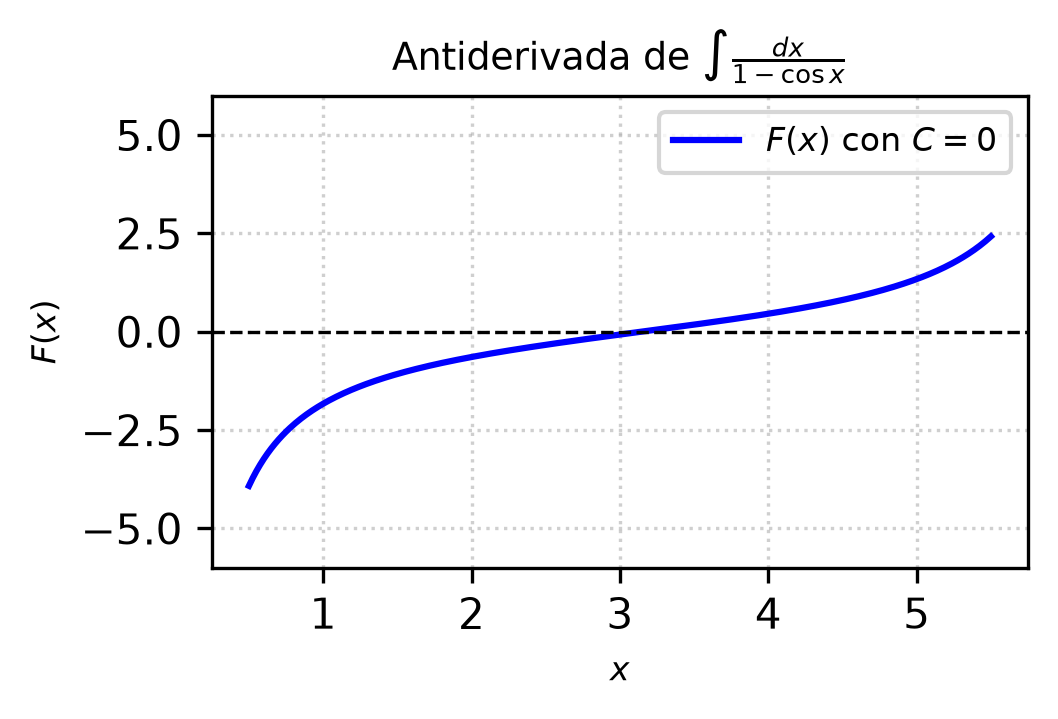
\includegraphics[width=\columnwidth]{semana_04/graficas/SEM04_P05_grafica.png}
	\caption{Representación gráfica de $f(x)$ y su antiderivada $F(x)$ evaluada para la constante de integración $C = 0$ (Problema 05).}
	\label{fig:problema05}
\end{figure}
